\documentclass{article}
\usepackage[landscape]{geometry}
\usepackage{url}
\usepackage{multicol}
\usepackage{amsmath}
\usepackage{esint}
\usepackage{amsfonts}
\usepackage{tikz}
\usetikzlibrary{decorations.pathmorphing}
\usepackage{amsmath,amssymb}
\usepackage{physics}
\usepackage{colortbl}
\usepackage{xcolor}
\usepackage{mathtools}
\usepackage{amsmath,amssymb}
\usepackage{enumitem}
\usepackage{graphicx}
\makeatletter

\newcommand*\bigcdot{\mathpalette\bigcdot@{.5}}
\newcommand*\bigcdot@[2]{\mathbin{\vcenter{\hbox{\scalebox{#2}{$\m@th#1\bullet$}}}}}
\makeatother

\title{130 Cheat Sheet}
\usepackage[brazilian]{babel}
\usepackage[utf8]{inputenc}

\advance\topmargin-.8in
\advance\textheight3in
\advance\textwidth3in
\advance\oddsidemargin-1.5in
\advance\evensidemargin-1.5in
\parindent0pt
\parskip2pt
\newcommand{\hr}{\centerline{\rule{3.5in}{1pt}}}
%\colorbox[HTML]{e4e4e4}{\makebox[\textwidth-2\fboxsep][l]{texto}
\begin{document}

\begin{center}{\huge{\textbf{PHYS 200 Final Cheat Sheet}}}\\
\end{center}
\begin{multicols*}{3}

\tikzstyle{mybox} = [draw=black, fill=white, very thick,
    rectangle, rounded corners, inner sep=10pt, inner ysep=10pt]
\tikzstyle{fancytitle} =[fill=black, text=white, font=\bfseries]

%------------ Heating ---------------
\begin{tikzpicture}
\node [mybox] (box){%
    \begin{minipage}{0.3\textwidth}
    $$E=\gamma mc^2, \vert \vec{p} \vert = \gamma mv \to E^2 = m^2 c^4 + p^2 c^2$$
    $$\vec{F} = \frac{d\vec{p}}{dt}$$
    LMatrix : $$\begin{bmatrix} \gamma & -\beta\gamma & 0 & 0 \\ -\beta\gamma & \gamma & 0 & 0 \\ 0 & 0 & 0 & 0 \\ 0 & 0 & 0 & 0 \end{bmatrix}$$

    \end{minipage}
};
%------------ Heating Header ---------------------
\node[fancytitle, right=10pt] at (box.north west) {Relativistic Dynamics};
\end{tikzpicture}

%------------ Mixing ---------------
\begin{tikzpicture}
\node [mybox] (box){%
    \begin{minipage}{0.3\textwidth}
      1. massless\\
      2. no rest frame $\rightarrow$  if had one, $E=0,p=0$ which is nothing.\\
      3. always move at $c$ (in all frames)\\
      4. $E=pc=hc/\lambda$, definite energy and momentum, related to \textbf{wavelength}
    \end{minipage}
};
%------------ Mixing Header ---------------------
\node[fancytitle, right=10pt] at (box.north west) {Photons};
\end{tikzpicture}

%------------ Inner Product Spaces ---------------
\begin{tikzpicture}
\node [mybox] (box){%
    \begin{minipage}{0.3\textwidth}
      1. Energy, momentum is always conserved $\rightarrow$ mass doens't have to be, can convert mass into KE\\
      2. Fusion: 2 light things $\rightarrow$ heavy thing + E \\
      3. Fission: 1 heavy thign $\rightarrow$ 2 (or more) lighter things + E \\
      4. Since stable is less energy state, we exert energy to go to stable state  \\
      5. In hydrogen atom $m_H = m_e + m_p - BE \to m_H  < m_e + m_p$ 
      
    \end{minipage}
};
%------------ Inner Product Space Header ---------------------
\node[fancytitle, right=10pt] at (box.north west) {Mass};
\end{tikzpicture}

%------------ Gram-Schmidt Content ---------------
\begin{tikzpicture}
\node [mybox] (box){%
    \begin{minipage}{0.3\textwidth}
    1. Move to center of mass frame (where stationary object decays). \\ 
    2. Compute momentum $\&$ energy, using LT revert back to original frame (be careful of sign).
    \end{minipage}
};
%------------ Gram-Schmidt Header ---------------------
\node[fancytitle, right=10pt] at (box.north west) {Particle decay, how to solve for diff frames};
\end{tikzpicture}
%------------ Variation of Parameters Content ---------------------
\begin{tikzpicture}
\node [mybox] (box){%
    \begin{minipage}{0.3\textwidth}
      $$\lambda' - \lambda = \frac{h}{m_e c}(1-\cos{\theta})$$
      1. $m$ is dependent on the object we are striking the photon to.\\
      2. Don't forget unit conversions. \\ 
      3. $hc = 1240 \text{nm}\cdot \text{eV}$
    \end{minipage}
};
%------------ Variation of Parameters Header ---------------------
\node[fancytitle, right=10pt] at (box.north west) {Compton Scattering};
\end{tikzpicture}

\begin{tikzpicture}
\node [mybox] (box){%
    \begin{minipage}{0.3\textwidth}
      $$\vec{E_0}\cos{kx-\omega t + \psi} \hspace{.2in} (k = 2\pi / \lambda , \omega = 2\pi f)$$  

\end{minipage}
};
%------------ ODE Header ---------------------
\node[fancytitle, right=10pt] at (box.north west) {Classical view};
\end{tikzpicture}



%------------ Systems of ODE Content ---------------
\begin{tikzpicture}
\node [mybox] (box){%
    \begin{minipage}{0.3\textwidth}
    1. $c=hf$ \\ 
    2. Energy is proportional to $E_0^2,B_0^2$ \\ 
    3. Intensity $\propto (E_0)^2$ a.k.a Probability $\propto (E_0)^2 \text{ and } I$
    4. Intensity = energy / (area * time), not dependent on frequency of light \\
    5. If intensity increase, it is related to the number of photons
    \end{minipage}
};
%------------ Systems of ODE Header ---------------------
\node[fancytitle, right=10pt] at (box.north west) {Classical view continued};
\end{tikzpicture}

%------------ Exponentiation Content ---------------
\begin{tikzpicture}
\node [mybox] (box){%
    \begin{minipage}{0.3\textwidth}
    1. $E_\gamma = hf$ \\ 
    2. $KE_\text{max} = hf - W$ \\ 
    3. $W$ is same unless metal changes \\ 
    4. $eV_\text{stop} = KE_\text{max} = hf - W$ \\ 
    5. If retarding potential applied, it is not that electrons are not ejected,  
    it is because some ejected electrons can't make through
    \end{minipage}
};
%------------ Spring-Mass Header ---------------------
\node[fancytitle, right=10pt] at (box.north west) {Photo Electric Effect};
\end{tikzpicture}
\
%------------ Laplace Transforms Content ---------------
\begin{tikzpicture}
\node [mybox] (box){%
    \begin{minipage}{0.3\textwidth}
    1. Compton Scattering \\ 2. Photoelectric: not existence of effect, rather it is effect of retarding potential, nature that it's a hit or a miss and photon disappers after hitting 
    \\ 3. Blackbody radiation: When wavelength is low, radiation is not infinite. (related to cost of ejecting a high energy particle) 
  \end{minipage}
};
%------------ Laplace Transforms Header ---------------------
\node[fancytitle, right=10pt] at (box.north west) {QM effect of light};
\end{tikzpicture}
%------------ Gaussian Integral Content ---------------------
\begin{tikzpicture}
\node [mybox] (box){%
    \begin{minipage}{0.3\textwidth}
    1. Photon / electron has a probability of hitting part of screen \\ 
    2. Somehow each particle knows diffraction pattern. Somehow each particle passes through both slits at the same time \\ 
    3. We don't know till measure \\ 
    4. hit screen at certain point (particle behav.), interference (with itself) pattern (wave behaviour) \\ 
    5. After measurement (position checked), position collapses and has definite position. 
    6. Before measurement, no position is known (only a probability distribution is known)
    \end{minipage}
};
%------------ Gaussian Integral Header ---------------------
\node[fancytitle, right=10pt] at (box.north west) {Diffraction pattern};
\end{tikzpicture}
%------------ Complex Numbers Content ---------------------
\begin{tikzpicture}
\node [mybox] (box){%
    \begin{minipage}{0.3\textwidth}

      1. Intensity $\propto$ E-field squared, thus probability $\propto$ wave amplitude squared \\ 
      2. $P(x) = \vert \psi(x) \vert ^2 = \psi(x) \bar{\psi(x)}$
	\end{minipage}
};
%------------ Gaussian Integral Header ---------------------
\node[fancytitle, right=10pt] at (box.north west) {Probability};
\end{tikzpicture}

%------------ Vector Spaces ---------------
\begin{tikzpicture}
\node [mybox] (box){%
    \begin{minipage}{0.3\textwidth} 
    1. Measurement : process through which observales is determined / recorded (position, momentum recorded) \\ 
    2. Eigenstate : A quantum state with 100 percent certainty  \\
    3. Quamtum superposition : Combination of different eigenstates with complex coefficients \\ 
    4. State : complete description of properties at some moment in time
  \end{minipage}
};
%------------ Vector Space Header ---------------------
\node[fancytitle, right=10pt] at (box.north west) {Terminlogies};
\end{tikzpicture}

\begin{tikzpicture}
\node [mybox] (box){%
    \begin{minipage}{0.3\textwidth} 
      1. $\sum_{\forall x}c(x) \ket{x} \equiv \int_{-\infty}^{\infty}c(x) \ket{x} dx$ \\ 
      2. $\ket{\psi(x)} = \int_{\infty}^{\infty} \psi(x) \ket{x}dx$  \\ 
      3. After measurement, state changes to appropriate eigen state \\ 
      4. If repeated measurement right after, get same result (system still in that eigenstate) \\ 
      5. If asked about diff measurement, we have to change basis i.e. new eigenstate \\ 
      6. Given $a_1\ket{x_1} + a_2\ket{x_2}$, a particle DOES NOT have a definite state.
    \end{minipage}
};
%------------ Vector Space Header ---------------------
\node[fancytitle, right=10pt] at (box.north west) {QM / Measurements};
\end{tikzpicture}

\begin{tikzpicture}
\node [mybox] (box){%
    \begin{minipage}{0.3\textwidth} 
      1. $\ket{\theta} = \cos{\theta} \ket{0} + \sin{\theta} \ket{90}$ \\ 
      2. probability transmission : $\cos^2{\theta}$ \\ 
      3. probability absorbed : $\sin^2{\theta}$ \\ 
      4. In case of $\ket{\phi} = a \ket{x} + b \ket{y}$, when getting probability need to normalize $\vert a\vert ^ 2+ \vert b \vert ^2 = 1$ \\ 
      5. Energy is still maintained.
      
    \end{minipage}
    
};
%------------ Vector Space Header ---------------------
\node[fancytitle, right=10pt] at (box.north west) {Polarization};
\end{tikzpicture}

\begin{tikzpicture}
\node [mybox] (box){%
    \begin{minipage}{0.3\textwidth} 
    1. For any particle, $pc = hc / \lambda \implies p = h / \lambda$. \\ 
    2. Use $e^{i2\pi p x / h}$ \\ 
    3. $\psi(x) = \frac{1}{\sqrt{h}} \int{\tilde{\psi}(p) e^{ipx/ \hbar}dp}$ \\ 
    4. $\tilde{\psi(p)}=\frac{1}{\sqrt{h}} \int{\psi(x)e^{-ipx/\hbar}dx}$ \\ 
  5. For post-measurement, $\psi(x) = e^{ip_0 x/\hbar},\tilde{\psi}(p)= e^{-ip x_0 /\hbar}$, cannot be properly normalized \\
    6. $\psi(R,t) = e^{2\pi i (R/ \lambda - ft)}, \hspace{.1in} R \approx D + \frac{Y^2}{2D}$ \\ 
    7. $\langle  x \rangle = \int_{-\infty}^{\infty} xP(x)dx= \int_{-\infty}^{\infty} x \vert \Psi(x) \vert^2 dx$ \\ 
    8. $\hbar = \frac{h}{2\pi}$, heisenberg uncertainty: $\Delta x \Delta p \geq \hbar / 2$
  \end{minipage}
};

%------------ Vector Space Header ---------------------
\node[fancytitle, right=10pt] at (box.north west) {De broglie wave length / others};
\end{tikzpicture}

\pagebreak


\begin{tikzpicture}
\node [mybox] (box){%
    \begin{minipage}{0.3\textwidth} 
      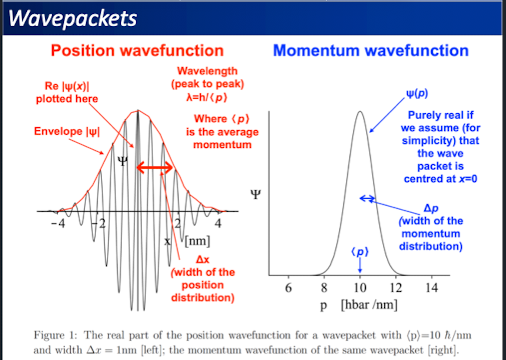
\includegraphics[width=\linewidth]{wavepacketimg.png} \\ 
      1. Wavepackets are needed to localize real wavefunctions (which are not as shown above) \\
      2. The narrower the wavepacket in position, wider range of frequencies, wider momentum wavefunction \\ 
      3. The narrower the wavepacket in momentum, the wider position wavefunction. \\ 
      4. $\langle p \rangle = \int_{-\infty}^{\infty} p \vert \tilde{\Psi}(p) \vert^2 dp$ \\ 
      5. $ (\Delta p)^2 = \int_{-\infty}^{\infty} (p - \langle p \rangle )^2 \vert \tilde{\Psi}(x) \vert^2 dp$ (Same for $x$)
    \end{minipage}
};

%------------ Vector Space Header ---------------------
\node[fancytitle, right=10pt] at (box.north west) {Wave Packets};
\end{tikzpicture}




\begin{tikzpicture}
\node [mybox] (box){%
    \begin{minipage}{0.3\textwidth} 
      $$c= 3.00 \times 10^8 \text{ms}^{-1}, \hspace{.3in} e = 1.60 \times 10^{-19}C $$ $$ h = 6.626 \times 10^{-34} \text{Js}$$
      $$m_e = 9.11 \times 10^{-31} \text{kg} , \hspace{.2in} m_p = 1.67 \times 10^{-27} \text{kg}$$
      $$m_{\pi_0} = 2.406 \times 10^{-28}\text{kg },u_x' = \frac{u_x - v}{1 - u_xv/c^2}$$
      $$\mathbf{P} = (\gamma(u)mc, \gamma(u)m\vec{u})= (E/c,\vec{p})$$
      $$1J = 6.242\times 10^{18}eV$$ \\ 
      1. Bound system has binding energy. Stable so low E. \\ 
      2. Bound system's mass is less than the sum of the masses of the components. \\ 
      3. Unstable bound system has sum of masses heavier than its components. \\ 
      4. Having half vertical and half horizontal polarized light is different from $\frac{1}{\sqrt{2}} \ket{0} + \frac{1}{\sqrt{2}} \ket{90}$ \\ 
      5. Bright fringes : $\frac{dY}{D} = m\lambda$, $d:\text{slit size}, D: \text{ Distance to screen}, Y: \text{ Height}$
    \end{minipage}
};

%------------ Vector Space Header ---------------------
\node[fancytitle, right=10pt] at (box.north west) {Constants, Formulae and others};

\end{tikzpicture}

\begin{tikzpicture}
\node [mybox] (box){%
    \begin{minipage}{0.3\textwidth} 
    1. A wavefunction of a moving free particle with a well defined momentum is simply a travelling wave \\ 
    $$e^{(i/\hbar)(px-Et)}$$
    2. $E= 1/2mv^2 = p^2/2m$ (non-relativistic) \\
    3. Time evolution for each component in a quamtum superposition happens independently
    
    \end{minipage}
};

%------------ Vector Space Header ---------------------
\node[fancytitle, right=10pt] at (box.north west) {Time evolution};


\end{tikzpicture}

\begin{tikzpicture}
\node [mybox] (box){%
    \begin{minipage}{0.3\textwidth} 
    1. Event : something that happens at some place ($x$) and some time ($t$) \\
    2. Relativity of Simultaneity: Events in another frame won't be simulatenous. \\ 
    3. Lengths perpendicular to motion do not change in length. \\ 
    4. All observers have to agree to some event, whether happening at the same time doesn't matter.
    \end{minipage}
};

%------------ Vector Space Header ---------------------
\node[fancytitle, right=10pt] at (box.north west) {Basics};


\end{tikzpicture}

\begin{tikzpicture}
\node [mybox] (box){%
    \begin{minipage}{0.3\textwidth} 
    $$T' = \frac{1}{\sqrt{1-(v/c)^2}}T = \gamma T$$
   Where $T$ is proper time, moving clock moves slower. \\ 
   Clock is synchronized from another frame. \\  
    \end{minipage}
};

%------------ Vector Space Header ---------------------
\node[fancytitle, right=10pt] at (box.north west) {Time Dilation};


\end{tikzpicture}


\begin{tikzpicture}
\node [mybox] (box){%
    \begin{minipage}{0.3\textwidth} 
      $$L' = \frac{1}{\gamma}L$$
      $L$ is proper length, as measured by observer in rest-frame of object. \\ 

    \end{minipage}
};

%------------ Vector Space Header ---------------------
\node[fancytitle, right=10pt] at (box.north west) {Length Contraction};


\end{tikzpicture}


\begin{tikzpicture}
\node [mybox] (box){%
    \begin{minipage}{0.3\textwidth} 
    Gallelian transformations fail at high speeds. \\ 
    $t' = \gamma (t- \frac{vx}{c^2}),\hspace{.2in}x'=\gamma (x - vt)$ \\ 
    $t = \gamma (t' + \frac{vx'}{c^2}),\hspace{.2in} x=\gamma (x'+vt')$ \\ ``
    Be careful of $v$ sign!!! Extra terms are for clock synchronization. \\ 
    Origins have to agree at the same place (think of Thanos!). \\ 
    $u'_x = \frac{u_x - V}{1 - u_xV/c^2},u_x = \frac{u'_x + V}{1 + u'_xV/c^2}$ \\ 
    $u'_y = \frac{u_y}{\gamma_v(1-u_xv/c^2)},u'_z= \frac{u_z}{\gamma_v(1-u_xv/c^2)}$
    \end{minipage}
};

%------------ Vector Space Header ---------------------
\node[fancytitle, right=10pt] at (box.north west) {Lorentz Transformations};


\end{tikzpicture}


\begin{tikzpicture}
\node [mybox] (box){%
    \begin{minipage}{0.3\textwidth} 
    $$(\Delta s)^2= -(c\Delta t)^2 + (\Delta x)^2 + (\Delta y)^2 + (\Delta z)^2$$
    This is lorentz invariant, $(\Delta s)^2 = (\Delta s')^2$ \\ 
    For two given events, any two inertial observers agree on $s^2$. \\
    Proper time: time measure between two events happening at same place ($\Delta x = 0$).  \\ 
    Proper length: length measure between two events happening at same time ($\Delta t = 0$). \\ 
    \end{minipage}
};

%------------ Vector Space Header ---------------------
\node[fancytitle, right=10pt] at (box.north west) {Space Time Interval};


\end{tikzpicture}


\begin{tikzpicture}
\node [mybox] (box){%
    \begin{minipage}{0.3\textwidth} 
    space-like separated: $(\Delta s)^2 = -(c\Delta t)^2 + (\Delta x)^2 > 0$ \\ 
    time-like separated: $(\Delta s)^2 = -(c\Delta t)^2 + (\Delta x)^2 < 0$ \\ 
    null-like separated: $(\Delta s)^2 = -(c\Delta t)^2 + (\Delta x)^2 = 0$ \\ 
    An event, would be a coordinate in the diagram (axes change per frame). \\ 
    In time-like separated, some events can happen at same place. \\ 
    In space-like separated, some evetns can happen at same time (or even reverse time).
  \end{minipage}
};

%------------ Vector Space Header ---------------------
\node[fancytitle, right=10pt] at (box.north west) {Space time diagram, Causality};


\end{tikzpicture}

\begin{tikzpicture}
\node [mybox] (box){%
    \begin{minipage}{0.3\textwidth} 
    We know that $\frac{\lambda}{p}$ and $f = \frac{E}{h}$ hence,
    $$e^{i(2\pi x/\lambda - 2\pi ft)} = e^{i(px - Et)/\hbar}$$
    $v_{\text{wave.propagation}} = \lambda f = E/p = (\frac{1}{2}mv^2)/(mv) = \frac{1}{2} $ \\ 
    $v_{wave packet} = \frac{df}{d(\lambda^{-1})} = \frac{d(E/h)}{d(p/h)} = dE/dp = \frac{d}{dp}(\frac{p^2}{2m}) = \frac{p}{m} = v$ \\ 
    dispersion : shorter wavelengths bunch at the the front, longer ones lag behind. \\
    Schrodinger Equation generates time evolution, 
    $$\frac{\partial \psi}{\partial t} = \frac{i\hbar}{2m}\frac{\partial^2 \psi}{\partial x^2}$$
    i.e. \\ 
    $$\psi(t+ \Delta t) \approx \psi(t) + \Delta t \frac{\partial \psi}{\partial t} = \psi(t) + \frac{i\hbar}{2m}\frac{\partial^2 \psi}{\partial x^2}\Delta t$$ 
    If we know $\psi$ for all $x$ at some $t$, we can solve for all $t$. 
    \end{minipage}
};

%------------ Vector Space Header ---------------------
\node[fancytitle, right=10pt] at (box.north west) {Schrodinger Equation};


\end{tikzpicture}


\begin{tikzpicture}
\node [mybox] (box){%
    \begin{minipage}{0.3\textwidth} 
      For a \textbf{free particle}, there is no force, momentum \textbf{does not change}. \\ 
      So if we measure position across some time, it is different (momentum!!) \\ 
      But if we measure momentum across some time, it is same! \\ 
      At the same time, energy is the same (if potential is same). \\ 
      For a free particle, S.E. is,
      $$i\hbar \frac{\partial}{\partial t} \psi(x,t) = -\frac{\hbar^2}{2m}\frac{\partial^2}{\partial x^2}\psi(x,t)$$
      If we have potential, then, 
      $$E= \frac{p^2}{2m}+V(x)$$
      and,
      $$i\hbar \frac{\partial \psi}{\partial t} = -\frac{\hbar^2}{2m}\frac{\partial ^2 \psi}{\partial x^2}+V(x)\psi$$
      Classically, an electron would bounce between bound states, but in QM the electron still would exist outside the bound! \\ 
      Now with potential, the width of the wavepacket wouldn't always increase. \\ 
      \textbf{Boundaries have to be continuous and approach 0 for $\pm \infty$}
    \end{minipage}
};

%------------ Vector Space Header ---------------------
\node[fancytitle, right=10pt] at (box.north west) {SE cont'd};
\end{tikzpicture}


\begin{tikzpicture}
\node [mybox] (box){%
    \begin{minipage}{0.3\textwidth} 
    Let's consider the SE with well-defined energy,
    $$i\hbar \frac{\partial}{\partial t}e^{-iEt/\hbar} = Ee^{-iEt/\hbar}$$
    Then,
    $$i\hbar \frac{\partial}{\partial t}(e^{-iEt/\hbar}\psi_E(x)=Ee^{-iEt/\hbar}\psi_E(x))$$
    This is a stationary state: PDF doesn't change with time.
  \end{minipage}
};

%------------ Vector Space Header ---------------------
\node[fancytitle, right=10pt] at (box.north west) {SE will well defined energy};

\end{tikzpicture}

\begin{tikzpicture}
\node [mybox] (box){%
    \begin{minipage}{0.3\textwidth} 
    Energy is also a classical observable, so there must exist states with well-defined energy. \\ 
    A.k.a \textbf{Energy Eigenstates} \\ 

    \end{minipage}
};

%------------ Vector Space Header ---------------------
\node[fancytitle, right=10pt] at (box.north west) {Energy Eigenstates};

\end{tikzpicture}

\begin{tikzpicture}
\node [mybox] (box){%
    \begin{minipage}{0.3\textwidth} 
      $$[-\frac{\hbar^2}{2m}\frac{\partial^2}{\partial x^2}+V(x)]e^{-iEt/\hbar \psi_E (x)} = Ee^{-iEt/\hbar}$$
      $$= Ee^{-iEt/\hbar}\psi_E(x)$$
      Hence,
      $$-\frac{\hbar^2}{2m}\frac{\partial^2}{\partial x^2}\psi_E(x)+V(x)\psi_E(x) = E\psi_E (x)$$
      \textbf{Solutions will only exist for discrete energies $\rightarrow$ energy spectrum. Solutions are called energy eigenstates.}
    \end{minipage}
};

%------------ Vector Space Header ---------------------
\node[fancytitle, right=10pt] at (box.north west) {Time independent SE};

\end{tikzpicture}


\begin{tikzpicture}
\node [mybox] (box){%
    \begin{minipage}{0.3\textwidth} 
      $$\psi_n = \sin(\frac{n\pi x}{L})$$
      $$E_n = \frac{\hbar^2}{2m}(\frac{n\pi}{L})^2 = \frac{h^2n^2}{8mL^2}$$

    \end{minipage}
};

%------------ Vector Space Header ---------------------
\node[fancytitle, right=10pt] at (box.north west) {Infinite Square Well};

\end{tikzpicture}

\begin{tikzpicture}
\node [mybox] (box){%
    \begin{minipage}{0.3\textwidth} 
    $V=0$ inside well, $V=V_0$ outside well. \\ 
    $$\frac{\partial^2 \psi}{\partial x^2}= \frac{2m}{\hbar^2}[V(x) - E]\psi$$
    If $E>V$ (inside well),
    $$\psi(x) = C \sin(k x) + D\cos(k x)$$
    If $E < V$ (inside barrier), 
    $$\psi(x) = Ae^{-kx}+Be^{kx}$$
    Depending on sign of $x$ either $A$ or $B$ can go to zero. \\ 
    Other constants can be determined by continuity of 0th, 1st derivative. \\ 
  \end{minipage}
};

%------------ Vector Space Header ---------------------
\node[fancytitle, right=10pt] at (box.north west) {Finite Square Well};

\end{tikzpicture}

\begin{tikzpicture}
\node [mybox] (box){%
    \begin{minipage}{0.3\textwidth} 
    Outside the well we get a function $e^{\pm \kappa x}$
    In anther way,
    $$e^{-x/ \eta} \rightarrow \eta = \frac{1}{\kappa} = \frac{\hbar}{\sqrt{2m(V-E)}}$$
    So now we have a finite chance of finding an electron outside of the well. \\ 
    Lowest energy is still not zero - electron always has some kinetic energy.
  \end{minipage}
};

%------------ Vector Space Header ---------------------
\node[fancytitle, right=10pt] at (box.north west) {Barrier Penetration};

\end{tikzpicture}

\begin{tikzpicture}
\node [mybox] (box){%
    \begin{minipage}{0.3\textwidth} 
    If the barrier isn't infinite width (would also work with infinite width), the wave would partially reflect and transmit at the same time. \\ 
    If we recall that $e^{-x/\eta}$ the bigger the difference between the potentail well height and particle energy, the less the wavefunction extends outside well. \\ 
    $$P_{\text{transmit}}=\lvert \Psi \rvert^2=(e^{-w/\eta})^2 = e^{-2w/\eta}$$
  \end{minipage}
};

%------------ Vector Space Header ---------------------
\node[fancytitle, right=10pt] at (box.north west) {Quantum Tunneling};

\end{tikzpicture}

\begin{tikzpicture}
\node [mybox] (box){%
    \begin{minipage}{0.3\textwidth} 
   time independent SE,
   $$-\frac{\hbar}{2m}(\partial_x^2+\partial_y^2+\partial_z^2)\psi_E - \frac{1}{4\pi\epsilon_0}\frac{e^2}{\lvert \vec{r} \rvert}\psi_E = E\psi_E $$ 
   $$E_n = - \frac{13.6\text{eV}}{n^2}$$
   An Hydrogen Atom is stable!, \\ 
   1. The electron isn't orbiting the nucleus, has a distributeed PDF centered on nucleus. \\ 
   2. Existence of lowest energy state implies stability (no lower state to go to). \\ 
   3. If atom radiates or absorbs photon, the electron jumps from one energy level to another (only certain frequencies are permitted (QM!)). 
   $$\lambda' = \gamma (1+ \frac{v}{c})\lambda$$
  \end{minipage}
};

%------------ Vector Space Header ---------------------
\node[fancytitle, right=10pt] at (box.north west) {Hydrogen Atom};

\end{tikzpicture}




\end{multicols*}
\end{document}


Contact GitHub API Training Shop Blog About
© 2016 GitHub, Inc. Terms Privacy Security Status Help
